\subsection{Polarización}

Se realizaron las mediciones de punto de polarización del amplificador sin señal aplicada, obteniéndose los resultados del cuadro~\tableref{tab:PuntoQ1}. Los mismos se verificaron con y sin la carga conectada para observar que no haya cambios en la polarización, una vez ajustada la corriente de polarización de salida, para este primer caso se ajustó la corriente de los transistores de salida en aproximadamente $190 \si[per-mode=symbol]{\milli\ampere}$. El segundo caso medido se muestra en el cuadro~\tableref{tab:PuntoQ2}, en este caso se ajusto la corriente al máximo que permite el preset del multiplicador de $V_{BE}$, aproximadamente $700 \si[per-mode=symbol]{\milli\ampere}$, como puede observarse en este caso la potencia disipada en reposo es considerable, unos $22 \si[per-mode=symbol]{\watt}$, pero puede verse como las primeras etapas prácticamente no se ven afectadas por el cambio en la corriente de reposo de los transistores de salida.


\vfill

\clearpage


\begin{table}[H]  %%\centering
    
    \setlength\arrayrulewidth{1.5pt}
    \arrayrulecolor{white}
    \def\clinecolor{\hhline{|>{\arrayrulecolor{white}}-%
    >{\arrayrulecolor{white}}|-|-|-|-|-|}}
    
\begin{center}  
\resizebox{0.7 \textwidth}{!}{%    
\begin{tabularx}{1 \textwidth}%
    {|
    >{\columncolor{white} \centering\arraybackslash}m{0.3333\linewidth}
     |
    >{\columncolor{white} \centering\arraybackslash}m{0.1667\linewidth}
     |
    >{\columncolor{white} \centering\arraybackslash}m{0.1667\linewidth}
     |
    >{\columncolor{white} \centering\arraybackslash}m{0.1667\linewidth}
     |
    >{\columncolor{white} \centering\arraybackslash}m{0.1667\linewidth}
     |
    }
    \rowcolor{HeadersColor} \thead{Transistor} & \thead{$V_{CE_{Q}}$} & \thead{$I_{C_{Q}}$} & \thead{ $P_{Q}$}\\    
    \hhline{|-|-|-|-|-|}
    %\rowcolor{Butter!20} \cellcolor{Butter!40} $I_{C}$ [$\si[per-mode=symbol]{\milli\ampere}$] & $0.54$ & $8.66$ & $9$ & $6$ & $5.5$ & $10$ & $10$  \\
    % \hhline{|-|-|-|-|-|}
    \rowcolor{gray!20} \cellcolor{gray!40} $Q_{1}$ (BC546C) & $33.87 \si[per-mode=symbol]{\volt}$  & $548.76 \si[per-mode=symbol]{\micro\ampere}$ & $ 18.57\si[per-mode=symbol]{\milli\watt}$ \\
    \hhline{|-|-|-|-|-|}
    \rowcolor{gray!20} \cellcolor{gray!40} $Q_{2}$ (BC556B) & $1.31 \si[per-mode=symbol]{\volt}$  & $548.76 \si[per-mode=symbol]{\milli\ampere}$ & $ 718.88\si[per-mode=symbol]{\micro\watt}$ \\
    \hhline{|-|-|-|-|-|}
    \rowcolor{gray!20} \cellcolor{gray!40} $Q_{3}$ (BC546B) & $31.78 \si[per-mode=symbol]{\volt}$  & $1.1 \si[per-mode=symbol]{\milli\ampere}$ & $ 34.96\si[per-mode=symbol]{\milli\watt}$ \\
    \hhline{|-|-|-|-|-|}
    \rowcolor{gray!20} \cellcolor{gray!40} $Q_{4}$ (BC556B) & $610.56 \si[per-mode=symbol]{\milli\volt}$  & $548.56 \si[per-mode=symbol]{\micro\ampere}$ & $ 334.93\si[per-mode=symbol]{\micro\watt}$ \\
    \hhline{|-|-|-|-|-|}
    \rowcolor{gray!20} \cellcolor{gray!40} $Q_{5}$ (BC546B) & $ 34.58 \si[per-mode=symbol]{\volt}$  & $548.56 \si[per-mode=symbol]{\micro\ampere}$ & $ 18.97\si[per-mode=symbol]{\milli\watt}$ \\
    \hhline{|-|-|-|-|-|}
    \rowcolor{gray!20} \cellcolor{gray!40} $Q_{6}$ (BC546B) & $29.02 \si[per-mode=symbol]{\volt}$  & $9.71 \si[per-mode=symbol]{\milli\ampere}$ & $ 281.78 \si[per-mode=symbol]{\milli\watt}$ \\
    \hhline{|-|-|-|-|-|}
    \rowcolor{gray!20} \cellcolor{gray!40} $Q_{7}$ (BC556B) & $30.32 \si[per-mode=symbol]{\volt}$  & $169.17 \si[per-mode=symbol]{\micro\ampere}$ & $ 5.13\si[per-mode=symbol]{\milli\watt}$ \\
    \hhline{|-|-|-|-|-|}
    \rowcolor{gray!20} \cellcolor{gray!40} $Q_{8}$ (BC556B) & $30.86 \si[per-mode=symbol]{\volt}$  & $9.55 \si[per-mode=symbol]{\milli\ampere}$ & $ 295.55\si[per-mode=symbol]{\milli\watt}$ \\
    \hhline{|-|-|-|-|-|}
    \rowcolor{gray!20} \cellcolor{gray!40} $Q_{9}$ (BD135) & $2.71 \si[per-mode=symbol]{\volt}$  & $9.46 \si[per-mode=symbol]{\milli\ampere}$ & $ 25.64\si[per-mode=symbol]{\milli\watt}$ \\
    \hhline{|-|-|-|-|-|}
    \rowcolor{gray!20} \cellcolor{gray!40} $Q_{10}$(BD136) & $14.09 \si[per-mode=symbol]{\volt}$  & $8.28 \si[per-mode=symbol]{\milli\ampere}$ & $ 116.67\si[per-mode=symbol]{\milli\watt}$ \\
    \hhline{|-|-|-|-|-|}
    \rowcolor{gray!20} \cellcolor{gray!40} $Q_{11}$(BD136) & $20.26 \si[per-mode=symbol]{\volt}$  & $0 \si[per-mode=symbol]{\milli\ampere}$ & $ 0\si[per-mode=symbol]{\milli\watt}$ \\
    \hhline{|-|-|-|-|-|}
    \rowcolor{gray!20} \cellcolor{gray!40} $Q_{12}$(BD135) & $20.27 \si[per-mode=symbol]{\volt}$  & $0 \si[per-mode=symbol]{\milli\ampere}$ & $ 0\si[per-mode=symbol]{\milli\watt}$ \\
    \hhline{|-|-|-|-|-|}
    \rowcolor{gray!20} \cellcolor{gray!40} $Q_{13}$(BD135) & $14.06 \si[per-mode=symbol]{\volt}$  & $9.7 \si[per-mode=symbol]{\milli\ampere}$ & $ 136.38 \si[per-mode=symbol]{\milli\watt}$ \\
    \hhline{|-|-|-|-|-|}
    \rowcolor{gray!20} \cellcolor{gray!40} $Q_{14}$(MJL21194) & $20.27 \si[per-mode=symbol]{\volt}$  & $0 \si[per-mode=symbol]{\milli\ampere}$ & $ 0\si[per-mode=symbol]{\milli\watt}$ \\
    \hhline{|-|-|-|-|-|}
    \rowcolor{gray!20} \cellcolor{gray!40} $Q_{15}$(MJL21194) & $14.72 \si[per-mode=symbol]{\volt}$  & $192.02 \si[per-mode=symbol]{\milli\ampere}$ & $ 2.83 \si[per-mode=symbol]{\watt}$ \\
    \hhline{|-|-|-|-|-|}
    \rowcolor{gray!20} \cellcolor{gray!40} $Q_{16}$(MJL21193) & $14.71 \si[per-mode=symbol]{\volt}$  & $193.5 \si[per-mode=symbol]{\milli\ampere}$ & $ 2.85 \si[per-mode=symbol]{\watt}$ \\
    \hhline{|-|-|-|-|-|}
    \rowcolor{gray!20} \cellcolor{gray!40} $Q_{17}$(MJL21193) & $20.26 \si[per-mode=symbol]{\volt}$  & $0 \si[per-mode=symbol]{\milli\ampere}$ & $ 0\si[per-mode=symbol]{\milli\watt}$ \\
    \hhline{|-|-|-|-|-|}
    \rowcolor{gray!20} \cellcolor{gray!40} $Q_{18}$(2N3906) & $1.36 \si[per-mode=symbol]{\volt}$  & $0 \si[per-mode=symbol]{\milli\ampere}$ & $ 0\si[per-mode=symbol]{\milli\watt}$ \\
    \hhline{|-|-|-|-|-|}
    \rowcolor{gray!20} \cellcolor{gray!40} $Q_{19}$(2N3904) &$1.35 \si[per-mode=symbol]{\volt}$  & $0 \si[per-mode=symbol]{\milli\ampere}$ & $ 0\si[per-mode=symbol]{\milli\watt}$ \\
    \hhline{|-|-|-|-|-|}            
    \end{tabularx}}
	\caption{Primer punto de operación.}
    \label{tab:PuntoQ1}
	\end{center}
\end{table}


\begin{table}[H]  %%\centering
    
    \setlength\arrayrulewidth{1.5pt}
    \arrayrulecolor{white}
    \def\clinecolor{\hhline{|>{\arrayrulecolor{white}}-%
    >{\arrayrulecolor{white}}|-|-|-|-|-|}}
    
\begin{center}  
\resizebox{0.7 \textwidth}{!}{%    
\begin{tabularx}{1 \textwidth}%
    {|
    >{\columncolor{white} \centering\arraybackslash}m{0.3333\linewidth}
     |
    >{\columncolor{white} \centering\arraybackslash}m{0.1667\linewidth}
     |
    >{\columncolor{white} \centering\arraybackslash}m{0.1667\linewidth}
     |
    >{\columncolor{white} \centering\arraybackslash}m{0.1667\linewidth}
     |
    >{\columncolor{white} \centering\arraybackslash}m{0.1667\linewidth}
     |
    }
    \rowcolor{HeadersColor} \thead{Transistor} & \thead{$V_{CE_{Q}}$} & \thead{$I_{C_{Q}}$} & \thead{ $P_{Q}$}\\    
    \hhline{|-|-|-|-|-|}
    %\rowcolor{Butter!20} \cellcolor{Butter!40} $I_{C}$ [$\si[per-mode=symbol]{\milli\ampere}$] & $0.54$ & $8.66$ & $9$ & $6$ & $5.5$ & $10$ & $10$  \\
    \rowcolor{gray!20} \cellcolor{gray!40} $Q_{1}$ (BC546C) & $33.87 \si[per-mode=symbol]{\volt}$  & $548.76 \si[per-mode=symbol]{\micro\ampere}$ & $ 18.57\si[per-mode=symbol]{\milli\watt}$ \\
    \hhline{|-|-|-|-|-|}
    \rowcolor{gray!20} \cellcolor{gray!40} $Q_{2}$ (BC556B) & $1.31 \si[per-mode=symbol]{\volt}$  & $548.76 \si[per-mode=symbol]{\milli\ampere}$ & $ 718.88\si[per-mode=symbol]{\micro\watt}$ \\
    \hhline{|-|-|-|-|-|}
    \rowcolor{gray!20} \cellcolor{gray!40} $Q_{3}$ (BC546B) & $31.78 \si[per-mode=symbol]{\volt}$  & $1.1 \si[per-mode=symbol]{\milli\ampere}$ & $ 34.96\si[per-mode=symbol]{\milli\watt}$ \\
    \hhline{|-|-|-|-|-|}
    \rowcolor{gray!20} \cellcolor{gray!40} $Q_{4}$ (BC556B) & $610.56 \si[per-mode=symbol]{\milli\volt}$  & $548.56 \si[per-mode=symbol]{\micro\ampere}$ & $ 334.93\si[per-mode=symbol]{\micro\watt}$ \\
    \hhline{|-|-|-|-|-|}
    \rowcolor{gray!20} \cellcolor{gray!40} $Q_{5}$ (BC546B) & $ 34.58 \si[per-mode=symbol]{\volt}$  & $548.56 \si[per-mode=symbol]{\micro\ampere}$ & $ 18.97\si[per-mode=symbol]{\milli\watt}$ \\
    \hhline{|-|-|-|-|-|}
    \rowcolor{gray!20} \cellcolor{gray!40} $Q_{6}$ (BC546B) & $28.79 \si[per-mode=symbol]{\volt}$  & $9.71 \si[per-mode=symbol]{\milli\ampere}$ & $ 279.55 \si[per-mode=symbol]{\milli\watt}$ \\
    \hhline{|-|-|-|-|-|}
    \rowcolor{gray!20} \cellcolor{gray!40} $Q_{7}$ (BC556B) & $30.05 \si[per-mode=symbol]{\volt}$  & $169.4 \si[per-mode=symbol]{\micro\ampere}$ & $ 5.09\si[per-mode=symbol]{\milli\watt}$ \\
    \hhline{|-|-|-|-|-|}
    \rowcolor{gray!20} \cellcolor{gray!40} $Q_{8}$ (BC556B) & $30.72 \si[per-mode=symbol]{\volt}$  & $9.57 \si[per-mode=symbol]{\milli\ampere}$ & $ 294 \si[per-mode=symbol]{\milli\watt}$ \\
    \hhline{|-|-|-|-|-|}
    \rowcolor{gray!20} \cellcolor{gray!40} $Q_{9}$ (BD135) & $2.95 \si[per-mode=symbol]{\volt}$  & $9.40 \si[per-mode=symbol]{\milli\ampere}$ & $ 27.73 \si[per-mode=symbol]{\milli\watt}$ \\
    \hhline{|-|-|-|-|-|}    
    \rowcolor{gray!20} \cellcolor{gray!40} $Q_{10}$(BD136) & $13.93 \si[per-mode=symbol]{\volt}$  & $14.73 \si[per-mode=symbol]{\milli\ampere}$ & $ 205.19 \si[per-mode=symbol]{\milli\watt}$ \\
    \hhline{|-|-|-|-|-|}
    \rowcolor{gray!20} \cellcolor{gray!40} $Q_{11}$(BD136) & $20.32 \si[per-mode=symbol]{\volt}$  & $0 \si[per-mode=symbol]{\milli\ampere}$ & $ 0\si[per-mode=symbol]{\milli\watt}$ \\
    \hhline{|-|-|-|-|-|}
    \rowcolor{gray!20} \cellcolor{gray!40} $Q_{12}$(BD135) & $20.30 \si[per-mode=symbol]{\volt}$  & $0 \si[per-mode=symbol]{\milli\ampere}$ & $ 0\si[per-mode=symbol]{\milli\watt}$ \\
    \hhline{|-|-|-|-|-|}
    \rowcolor{gray!20} \cellcolor{gray!40} $Q_{13}$(BD135) & $13.89 \si[per-mode=symbol]{\volt}$  & $18.66 \si[per-mode=symbol]{\milli\ampere}$ & $ 259.19 \si[per-mode=symbol]{\milli\watt}$ \\
    \hhline{|-|-|-|-|-|}
    \rowcolor{gray!20} \cellcolor{gray!40} $Q_{14}$(MJL21194) & $20.32 \si[per-mode=symbol]{\volt}$  & $0 \si[per-mode=symbol]{\milli\ampere}$ & $ 0\si[per-mode=symbol]{\milli\watt}$ \\
    \hhline{|-|-|-|-|-|}
    \rowcolor{gray!20} \cellcolor{gray!40} $Q_{15}$(MJL21194) & $14.62 \si[per-mode=symbol]{\volt}$  & $700.06 \si[per-mode=symbol]{\milli\ampere}$ & $ 10.23 \si[per-mode=symbol]{\watt}$ \\
    \hhline{|-|-|-|-|-|}
    \rowcolor{gray!20} \cellcolor{gray!40} $Q_{16}$(MJL21193) & $14.61 \si[per-mode=symbol]{\volt}$  & $704.1 \si[per-mode=symbol]{\milli\ampere}$ & $ 10.29 \si[per-mode=symbol]{\watt}$ \\
    \hhline{|-|-|-|-|-|}    
    \rowcolor{gray!20} \cellcolor{gray!40} $Q_{17}$(MJL21193) & $20.32 \si[per-mode=symbol]{\volt}$  & $0 \si[per-mode=symbol]{\milli\ampere}$ & $ 0\si[per-mode=symbol]{\milli\watt}$ \\
    \hhline{|-|-|-|-|-|}
    \rowcolor{gray!20} \cellcolor{gray!40} $Q_{18}$(2N3906) & $1.47 \si[per-mode=symbol]{\volt}$  & $0 \si[per-mode=symbol]{\milli\ampere}$ & $ 0\si[per-mode=symbol]{\milli\watt}$ \\
    \hhline{|-|-|-|-|-|}
    \rowcolor{gray!20} \cellcolor{gray!40} $Q_{19}$(2N3904) & $1.48 \si[per-mode=symbol]{\volt}$  & $0 \si[per-mode=symbol]{\milli\ampere}$ & $ 0\si[per-mode=symbol]{\milli\watt}$ \\
    \hhline{|-|-|-|-|-|}            
    \end{tabularx}}
	\caption{Segundo punto de operación.}
    \label{tab:PuntoQ2}
	\end{center}
\end{table}


\vfill

\clearpage



\subsection{Ancho de banda}

\par Para la medición del ancho de banda, se buscaron las frecuencias de corte para una señal tal que sea el $10 \si[per-mode=symbol]{\percent}$ de la potencia máxima de $40 \si[per-mode=symbol]{\watt}$ especificada. Por lo tanto, se obtiene que la tensión de salida deberá tener un valor de $v_{out} = 8.9 \si[per-mode=symbol]{\volt}$, y las frecuencias de corte se determinaran cuando $v_{out} \approx 8.48 \si[per-mode=symbol]{\volt}$.

\par Se pueden observar los resultados de la medición en el cuadro ~\tableref{tab:BW_low_power}.

\begin{table}[H]
    \centering
    \begin{tabular}{|c|c|c|c|} \hline
        Frecuencia & $V_{out}$ & $P$ & Fase \\ \hline
        $10 \si[per-mode=symbol]{\hertz}$      & $7.2 \si[per-mode=symbol]{\volt}$ & $3.24 \si[per-mode=symbol]{\watt}$ & $38.9 \si[per-mode=symbol]{\degree}$ \\ \hline
        $17.32 \si[per-mode=symbol]{\hertz}$   & $8.4 \si[per-mode=symbol]{\volt}$ & $4.41 \si[per-mode=symbol]{\watt}$ & $23.13^\circ$ \\ \hline
        $100 \si[per-mode=symbol]{\hertz}$     & $8.9 \si[per-mode=symbol]{\volt}$ & $5 \si[per-mode=symbol]{\watt}$ & - \\ \hline
        $1 \si[per-mode=symbol]{\kilo\hertz}$      & $8.9 \si[per-mode=symbol]{\volt}$ & $5 \si[per-mode=symbol]{\watt}$ & - \\ \hline
        $10 \si[per-mode=symbol]{\kilo\hertz}$     & $8.9 \si[per-mode=symbol]{\volt}$ & $5 \si[per-mode=symbol]{\watt}$ & - \\ \hline
        $42.3 \si[per-mode=symbol]{\kilo\hertz}$   & $8.4 \si[per-mode=symbol]{\volt}$ & $4.41 \si[per-mode=symbol]{\watt}$ & $0.12 \si[per-mode=symbol]{\degree}$ \\ \hline
        $100 \si[per-mode=symbol]{\kilo\hertz}$    & $8 \si[per-mode=symbol]{\volt}$   & $4 \si[per-mode=symbol]{\watt}$ & $29.52 \si[per-mode=symbol]{\degree}$ \\ \hline
    \end{tabular}
    \caption{Valores significativos del ancho de banda a baja potencia.}
    \label{tab:BW_low_power}
\end{table}

\par En el cuadro ~\tableref{tab:comp_BW_low_power} se comparan los ancho de banda obtenidos por simulación, los medidos y los especificados:

\begin{table}[H]
    \centering
    \begin{tabular}{|c|c|c|c|}
        Valor & Especificación & Simulación & Medición \\
        $f_{l}$ & $10 \si[per-mode=symbol]{\hertz}$ & $22.34 \si[per-mode=symbol]{\hertz}$ & $17.32 \si[per-mode=symbol]{\hertz}$ \\ \hline
        $f_{h}$ & $50 \si[per-mode=symbol]{\kilo\hertz}$ & $97.92 \si[per-mode=symbol]{\kilo\hertz}$ & $42.3 \si[per-mode=symbol]{\kilo\hertz}$ \\ \hline
    \end{tabular}
    \caption{Comparación de ancho de banda a baja potencia}
    \label{tab:comp_BW_low_power}
\end{table}

\par En la figura ~\figref{fig:BW_low_power_fl} se muestra la medición para el valor de $f_l$ para baja potencia, y en las figuras ~\figref{fig:BW_low_power_fl_phase} y ~\figref{fig:BW_low_power_fh_phase}, se muestran las mediciones para el cálculo de la fase de corrimiento de las señales.


\begin{figure}[H]
    \centering
    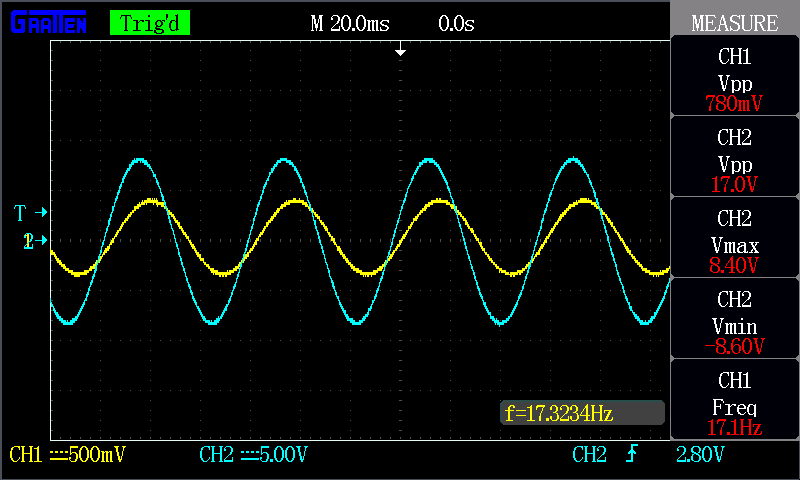
\includegraphics[scale=0.75]{./img/mediciones/BW_low_power/1.png}
    \caption{Medición de $f_{l}$ a baja potencia, mostrando el corrimiento de fase.}
    \label{fig:BW_low_power_fl}
\end{figure}

\begin{figure}[H]
    \centering
    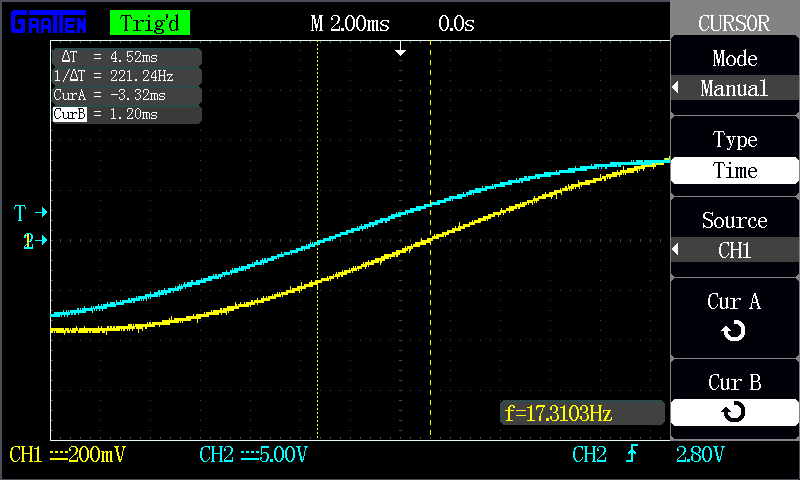
\includegraphics[scale=0.75]{./img/mediciones/BW_low_power/3.png}
    \caption{Cálculo del corrimiento de fase para $f_{l}$ a baja potencia.}
    \label{fig:BW_low_power_fl_phase}
\end{figure}

\begin{figure}[H]
    \centering
    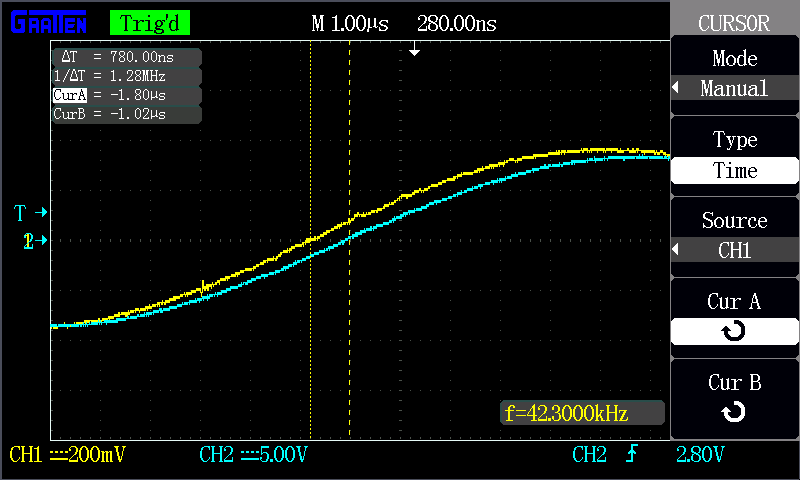
\includegraphics[scale=0.75]{./img/mediciones/BW_low_power/4.png}
    \caption{Cálculo del corrimiento de fase para $f_{h}$ a baja potencia.}
    \label{fig:BW_low_power_fh_phase}
\end{figure}



\subsection{Ancho de banda de potencia}

\par Para el caso del ancho de banda de potencia, se repite el procedimiento de la sección anterior pero con una señal de salida $V_{out} = 25.3 \si[per-mode=symbol]{\volt}$ a máxima potencia ($40 \si[per-mode=symbol]{\watt}$). En este caso, las frecuencias de corte se determinan cuando $V_{out} = 24 \si[per-mode=symbol]{\volt}$.
\par Se pueden observar los resultados de la medición en el cuadro ~\tableref{tab:BW_power}.

\begin{table}[H]
    \centering
    \begin{tabular}{|c|c|c|c|} \hline
        Frecuencia & $V_{out}$ & $P$ & Fase \\ \hline
        $10 \si[per-mode=symbol]{\hertz}$      & $20.8 \si[per-mode=symbol]{\volt}$ & $27.09 \si[per-mode=symbol]{\watt}$ & $49.32 \si[per-mode=symbol]{\degree}$ \\ \hline
        $19.75 \si[per-mode=symbol]{\hertz}$   & $24 \si[per-mode=symbol]{\volt}$ & $4.41 \si[per-mode=symbol]{\watt}$ & $24.56 \si[per-mode=symbol]{\degree}$ \\ \hline
        $100 \si[per-mode=symbol]{\hertz}$     & $25.3 \si[per-mode=symbol]{\volt}$ & $5 \si[per-mode=symbol]{\watt}$ & - \\ \hline
        $1 \si[per-mode=symbol]{\kilo\hertz}$      & $25.3 \si[per-mode=symbol]{\volt}$ & $5 \si[per-mode=symbol]{\watt}$ & - \\ \hline
        $10 \si[per-mode=symbol]{\kilo\hertz}$     & $25.3 \si[per-mode=symbol]{\volt}$ & $5 \si[per-mode=symbol]{\watt}$ & - \\ \hline
        $37.54 \si[per-mode=symbol]{\kilo\hertz}$   & $24 \si[per-mode=symbol]{\volt}$ & $4.41 \si[per-mode=symbol]{\watt}$ & $23.09 \si[per-mode=symbol]{\degree}$ \\ \hline
    \end{tabular}
    \caption{Valores significativos del ancho de banda a máxima potencia.}
    \label{tab:BW_power}
\end{table}

\par En el cuadro ~\tableref{tab:comp_BW_power} se comparan los anchos de banda obtenidos por simulación, los medidos y los especificados:

\begin{table}[H]
    \centering
    \begin{tabular}{|c|c|c|c|}
        Valor & Especificación & Simulación & Medición \\
        $f_l$ & $-$ & $22.34 \si[per-mode=symbol]{\hertz}$ & $19.75 \si[per-mode=symbol]{\hertz}$ \\ \hline
        $f_h$ & $30 \si[per-mode=symbol]{\kilo\hertz}$ & $97.84 \si[per-mode=symbol]{\kilo\hertz}$ & $37.54 \si[per-mode=symbol]{\kilo\hertz}$ \\ \hline
    \end{tabular}
    \caption{Comparación de ancho de banda a máxima potencia}
    \label{tab:comp_BW_power}
\end{table}




\par En las figuras ~\figref{fig:BW_power_fl_phase} y ~\figref{fig:BW_power_fh_phase}, se muestran las mediciones para el cálculo de la fase de corrimiento de las señales.



\begin{figure}[H]
    \centering
    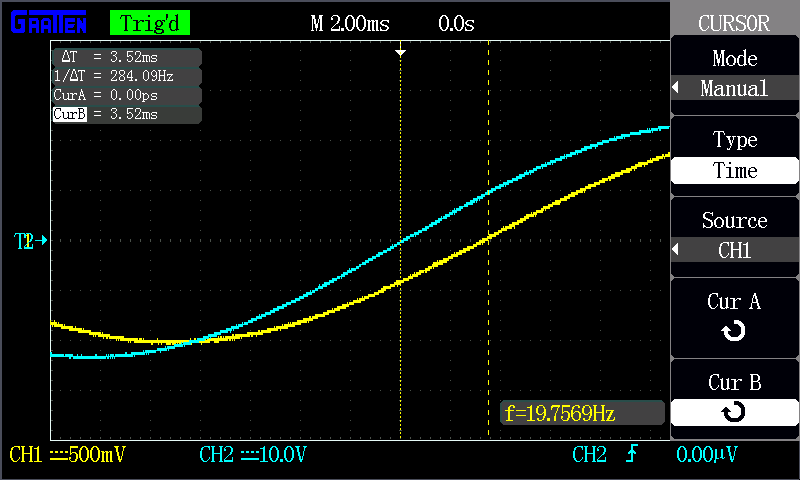
\includegraphics[scale=0.75]{./img/mediciones/BW_power/3.png}
    \caption{Medición de $f_l$ a máxima potencia, mostrando el corrimiento de fase.}
    \label{fig:BW_power_fl_phase}
\end{figure}


\begin{figure}[H]
    \centering
    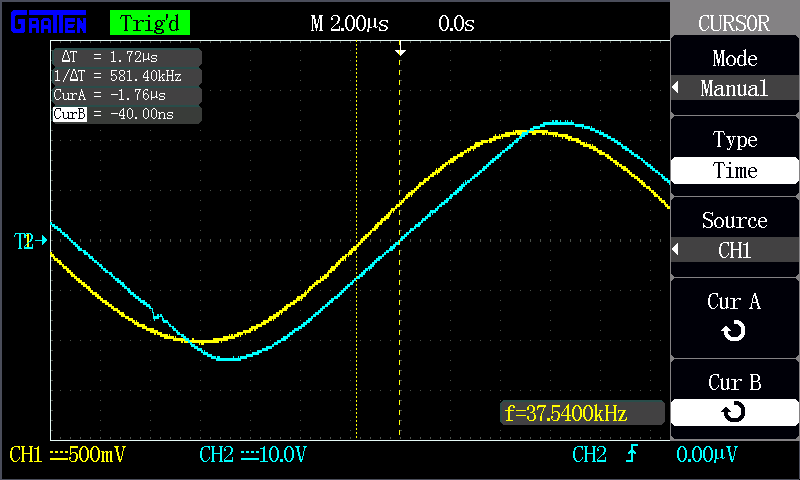
\includegraphics[scale=0.75]{./img/mediciones/BW_power/4.png}
    \caption{Medición de $f_l$ a máxima potencia, mostrando el corrimiento de fase.}
    \label{fig:BW_power_fh_phase}
\end{figure}





\subsection{Sensibilidad}

\par Se midió el valor eficaz de una señal senoidal de 1kHz aplicada a la entrada $v_{in}=1.08 \si[per-mode=symbol]{\volt}$, que produce la potencia especificada a la salida con carga nominal, siendo esta última $v_{out}= 25.2 \si[per-mode=symbol]{\volt}$. Se verifica dicha medición en la figura ~\figref{fig:Sensitivity}.

\begin{figure}[H]
    \centering
    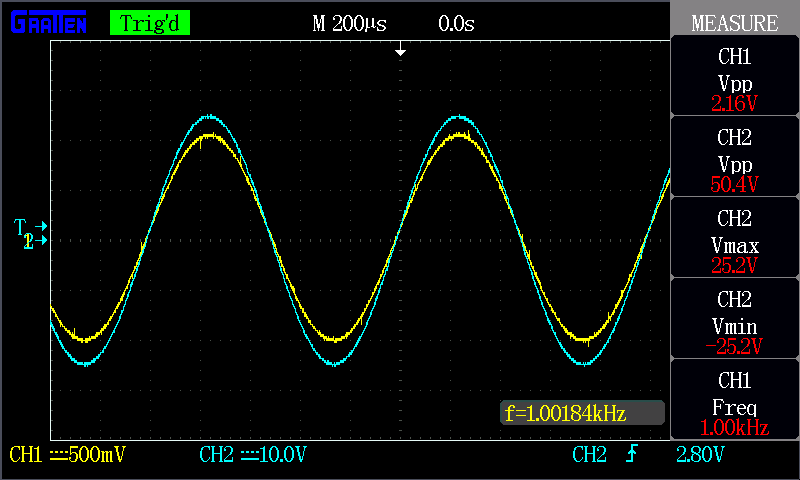
\includegraphics[scale=0.75]{./img/mediciones/Sensitivity/1.png}
    \caption{Medición de la sensibilidad del circuito amplificador.}
    \label{fig:Sensitivity}
\end{figure}


\subsection{THD}



\subsection{Slew Rate}

\par Se aplicó una señal cuadrada de máxima potencia a modo de obtener el valor numérico del SR, calculando la pendiente de la recta obtenida en la figura~\figref{fig:Slew_rate_amplifier}. Antes, se verficó en la figura  ~\figref{fig:Slew_rate_gen} que el tiempo de crecimiento de la fuente generadora de señal sea lo suficientemente baja para poder garantizar una correcta medición, siendo este tiempo de $\tau = 264 \si[per-mode=symbol]{\nano\second}$.


\begin{figure}[H]
        \centering
        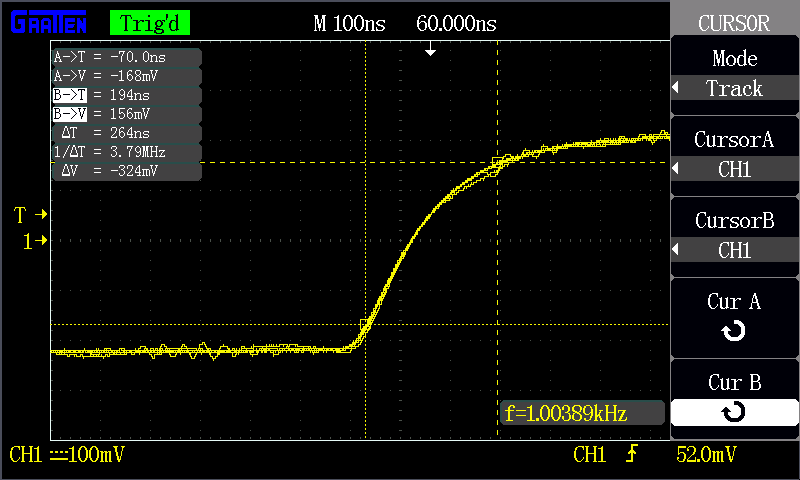
\includegraphics[scale=0.75]{./img/mediciones/Slew_Rate/1.png}
        \caption{Verificación de tiempo de crecimiento del generador.}
        \label{fig:Slew_rate_gen}
\end{figure}

\begin{figure}[H]
        \centering
        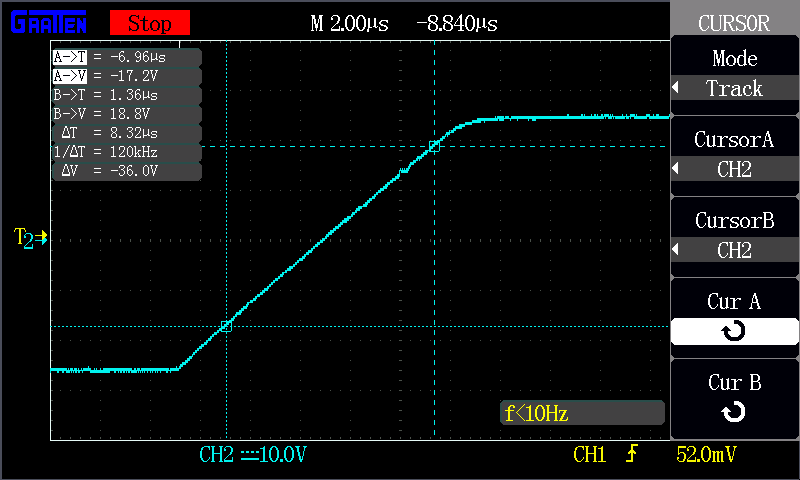
\includegraphics[scale=0.75]{./img/mediciones/Slew_Rate/2.png}
        \caption{Medición del Slew Rate del circuito amplificador.}
        \label{fig:Slew_rate_amplifier}
\end{figure}

\par Mediante el cálculo pertinente, y comparando con las simulaciones, se obtiene el cuadro comparativo  ~\tableref{tab:comp_SlewRate}:

\begin{table}[H]
    \centering
    \begin{tabular}{|c|c|c|c|}
        Valor & Especificación& Simulación & Medición \\
        \textit{Slew Rate} & $5 \si[per-mode=symbol]{\volt\per\micro\second}$ & $4.79 \si[per-mode=symbol]{\volt\per\micro\second}$ & $4.32 \si[per-mode=symbol]{\volt\per\micro\second}$ \\ \hline
    \end{tabular}
    \caption{Comparación del Slew Rate.}
    \label{tab:comp_SlewRate}
\end{table}

